\documentclass[12pt]{article}

\usepackage{makecell}

\usepackage[english]{babel}
\usepackage{datetime}

\title{\textbf{\textsf{Bitonic Sort on GPU \\ CUDA Implementations \& Optimizations}}}
\date{\monthname\ \the\year}

% math
\usepackage{amsmath, amssymb}
\usepackage{enumitem}
\usepackage{xcolor}

\usepackage{algorithm}        % For the algorithm environment
\usepackage{algpseudocode}    % For algorithmic commands and pseudocode formatting

\usepackage{ulem}

% references
\usepackage[style=apa, backend=biber]{biblatex}

% fonts
\usepackage{helvet}
\usepackage{sectsty}
\allsectionsfont{\sffamily} % for section titltes use sans-serif
% \renewcommand{\familydefault}{\sfdefault} % comment out for sans-serif font
% \usepackage{sansmath} % comment out for sans-serif math font
% \sansmath % comment out for sans-serif math font

% margins
\usepackage{geometry}
\geometry{
  a4paper,
  total={170mm,257mm},
  left=25mm,
  right=25mm,
  top=30mm,
  bottom=30mm,
}

% no indentation when a new paragraph starts
\setlength{\parindent}{0cm}

% links
\usepackage{hyperref} % better links
\usepackage{color}    % nicer link colors
\definecolor{pigment}{rgb}{0.2, 0.2, 0.6}
\hypersetup{
  colorlinks = true, % Color links instead of ugly boxes
  urlcolor   = pigment, % Color for external hyperlinks
  linkcolor  = black, % Color for internal links
  citecolor  = pigment % Color for citations
}

%%%%%%%%%%%%%%%%%%%%%%%%%%%%%%%%%%%%%%% headers  %%%%%%%%%%%%%%%%%%%%%%%%%%%%%%%%%%%%%%%
\usepackage{fancyhdr}
\pagestyle{fancy}
\lhead{Bitonic Sort with CUDA}
\chead{}
\rhead{Intro}

% example boxes
\usepackage{tcolorbox}
\newtcolorbox{examplebox}[1]{%
  colback=white,
  colframe=gray!30,
  title={#1},
  sharp corners,
  boxrule=0.5pt,
  coltitle=black
}


% conditionals
\usepackage{ifthen}
\newboolean{showinstructions}
\newboolean{showexamples}
\newboolean{showexplanations}
\renewenvironment{examplebox}[1]{%
  \ifthenelse{\boolean{showexamples}}%
    {\begin{tcolorbox}[colback=white, colframe=gray!30, title={#1}, sharp corners, boxrule=0.5pt, coltitle=black]}%
    {\expandafter\comment}%
}{%
  \ifthenelse{\boolean{showexamples}}%
    {\end{tcolorbox}}%
    {\expandafter\endcomment}%
}

% Define a new environment for explanations
\newcommand{\explanation}[1]{%
  \ifthenelse{\boolean{showexplanations}}%
    {\textit{Explanation:} #1}%
    {\ignorespaces}%
}

% Define a new environment for instructions
\newcommand{\instructions}[1]{%
  \ifthenelse{\boolean{showinstructions}}%
    {#1}%
    {\ignorespaces}%
}

\makeatletter
\newcommand{\maketitlepage}{%
    \begin{titlepage}
        \maketitle
        \thispagestyle{empty}
        \vfill 
        \centering
        \author{\textbf{Author: Aristeidis Daskalopoulos}} \\
        Github Repo: \url{https://github.com/arisdask/BitonicSortCUDA} \\ 
        \textit{A Parallel \& Distributed Systems' Project}
        \vfill 
    \end{titlepage}
    \newpage
}
\makeatother

% Optional user settings
\setboolean{showinstructions}{true} % set to false to hide instructions
\setboolean{showexamples}{true} % set to false to hide examples
\setboolean{showexplanations}{true} % set to false to hide explanations

\begin{document}
\maketitlepage

\instructions{\section{Intro}
\subsection*{Problem Introduction}
The primary objective of this project is to implement the Bitonic Sort algorithm using CUDA. This work presents three versions of the implementation, each serving as an optimization of the previous one. The Bitonic Sort algorithm is particularly well-suited for GPU execution due to its regular comparison patterns and parallelizable structure. The three versions progressively optimize the algorithm by reducing synchronization overhead and minimizing global memory accesses for improved performance.

\subsection*{Versions Implemented}
\begin{itemize}
    \item \textbf{V0 (Baseline Implementation)}: \\
    The initial version (V0) is a direct translation of the Bitonic Sort algorithm to CUDA, where each step of the algorithm is executed in a separate kernel function call. While simple to implement, V0 suffers from significant performance bottlenecks caused by the large number of kernel launches and inefficient (global) memory access, requiring explicit synchronization between steps, which further increases overhead.

    \item \textbf{V1 (Kernel Optimization)}: \\
    The second version (V1) optimizes V0 by fusing multiple steps of the Bitonic Sort algorithm into a single kernel. This reduces the number of kernel launches and minimizes the global synchronization overhead. This version is more efficient than V0, but it remains limited by global memory bandwidth, as \textit{all data exchanges still occur in global memory}.

    \item \textbf{V2 (Shared Memory Optimization)}: \\
    The third version (V2) introduces shared memory to further optimize the algorithm. By leveraging the GPU's faster on-chip memory, V2 minimizes global memory accesses by performing intermediate comparisons and exchanges in shared memory. This allows multiple comparison steps to be completed before writing results back to global memory, achieving the best performance among the three versions.
\end{itemize}

}

%%%%%%%%%%%%%%%%%%%%%%%%%%%%%%%%%%%%%%% headers  %%%%%%%%%%%%%%%%%%%%%%%%%%%%%%%%%%%%%%%
\pagestyle{fancy}
\lhead{Bitonic Sort with CUDA}
\chead{}
\rhead{Theoretical Algorithm Analysis}

\section{Theoretical Algorithm Analysis}
In this section, we introduce the bitonic sort algorithm that has been implemented. We explain its theoretical foundation, detailing how it functions step-by-step. Following this, we calculate its complexity and identify areas for optimization.

\subsection{First Algorithmic Approach (V0)}

The Bitonic Sort algorithm consists of multiple \textbf{stages} and \textbf{steps}. For an array of size \( N = 2^k \), the algorithm requires \( \log_2 N \) stages, and each stage \( s \in \{0, \dots, (\log_2 N) - 1\} \) consists of \( s + 1 \) steps. At each step, pairs of elements are \textit{compared} and \textit{swapped} based on their positions in the bitonic sequence.

\begin{algorithm}[H]
\caption{Bitonic Sort V0}\label{alg:v0}
\begin{algorithmic}[1]
\Require \textbf{Input}: Array \( \text{data} \) of size \( N = 2^k \)
\Ensure \textbf{Output}: Sorted array in ascending order

\State \( \text{stages} \gets \log_2 N \) \Comment{Total number of stages}
\For{\( \text{stage} = 0 \) to \( \text{stages} - 1 \)}
    \For{\( \text{step} = \text{stage} \) downto \( 0 \)}
        \State Launch CUDA kernel: \texttt{bitonic\_kernel\_v0}|parameters: \( (\text{data}, N, \text{stage}, \text{step}) \)
        \State Global Sync all threads \Comment{Ensure all threads complete the step}
    \EndFor
\EndFor
\end{algorithmic}
\end{algorithm}

The \texttt{bitonic\_kernel\_v0} is responsible for executing a single step of the Bitonic Sort algorithm. Here is the detailed algorithm of this kernel:


\begin{algorithm}[H]
\caption{bitonic\_kernel\_v0}\label{alg:v0_kernel}
\begin{algorithmic}[1]
\Require \textbf{Input}: 
    \( \text{\textbf{data}} \): Pointer to the array in global memory |  
    \( \text{\textbf{length}} \): Length of the array | 
    \( \text{\textbf{stage}} \): Current stage of the Bitonic Sort | 
    \( \text{\textbf{step}} \): Current step within the stage
\Ensure \textbf{Output}: Partially ``sorted" array after the current step (creates a bitonic sequence)

\State \( \text{tid} \gets \text{blockIdx.x} \times \text{blockDim.x} + \text{threadIdx.x} \) \Comment{Compute global thread ID}
\If{\( \text{tid} \geq (\text{length} \div 2) \)} 
    \State \Return \Comment{Exit if thread is out of bounds}
\EndIf

\State \( \text{idx} \gets \text{GET\_ARR\_ID}(\text{tid}, \text{step}) \) \Comment{Element index that this thread will handle}
\State \( \text{partner} \gets \text{idx} \oplus (1 \ll \text{step}) \) \Comment{Partner idx that this thread will handle (XOR)}

\If{\( \text{idx} < \text{partner} \land \text{partner} < \text{length} \)}
    \State \( \text{exchange}(\text{data}, \text{idx}, \text{idx}, \text{partner}, \text{stage}) \) \Comment{Compare and swap elements}
\EndIf
\end{algorithmic}
\end{algorithm}


\subsection{Explaining the Algorithm}
Here, we provide a detailed explanation of how the above algorithm works. We describe the key stages of the algorithm, the role of the kernel function, and how \texttt{GET\_ARR\_ID} \& data exchanges occur to achieve the final sorted outcome.

\subsubsection{Stages and Steps Overview}

For each stage \( s \) (from \( 0 \) to \( \log_2 N - 1 \)):
\begin{itemize}[nosep]
    \item For each step \( t \) (from \( s \) down to \( 0 \)):
    \begin{itemize}[nosep]
        \item Launch the \texttt{bitonic\_kernel\_v0} kernel.
        \item Each thread computes its element index using \texttt{GET\_ARR\_ID} and its partner index using XOR.
        \item The thread compares its element with its partner and swaps them if necessary.
        \item A global synchronization barrier ensures all threads complete the current step before proceeding.
        \begin{examplebox}{\textit{About Global Sync}}
            This synchronization is necessary to maintain the correctness of the Bitonic Sort algorithm, as \textit{each step depends on the results of the previous step}. 
            This means that after launching a kernel, the CPU must wait for the GPU to complete the kernel execution before launching the next kernel.
            
            However, we should keep in mind that frequent ``global" synchronization (between all threads) adds overhead and reduces performance.
        \end{examplebox}
    \end{itemize}
\end{itemize}


\subsubsection{Thread and Block Initialization in CUDA}

In CUDA, computation is divided into \textbf{threads} and \textbf{blocks}, which are organized in a grid. Proper initialization of threads and blocks is crucial for executing the Bitonic Sort algorithm efficiently. The following describes the initialization process in the \textbf{V0 implementation}.

\vspace{+5pt}

\textbf{\underline{\textit{Grid and Block Configuration}}}
\begin{itemize}[nosep]
    \item The grid consists of multiple blocks, each containing a fixed number of threads.
    \item The number of threads per block is defined by \texttt{THREADS\_PER\_BLOCK}, set to a power of two (e.g., 1024) to align with the GPU’s warp size (32 threads).
    \item The number of blocks is computed based on the input array size and the number of threads per block:
    \[
    \text{num\_blocks} = \left\lceil \frac{N / 2}{\text{THREADS\_PER\_BLOCK}} \right\rceil
    \]
    where \( N \) is the array size and \( N / 2 \) represents the number of element pairs to be processed (each thread handles the two partner-elements for the given \textit{step}).
\end{itemize}

\vspace{+5pt}

\textbf{\underline{\textit{Thread Initialization}}}
\begin{itemize}[nosep]
    \item Each thread computes its \textbf{global thread ID} as:
    \[
    \text{global\_tid} = \text{blockIdx.x} \times \text{blockDim.x} + \text{threadIdx.x}
    \]
    \begin{itemize}[nosep]
        \item \texttt{blockIdx.x}: Index of the block in the grid.
        \item \texttt{blockDim.x}: Number of threads per block.
        \item \texttt{threadIdx.x}: Index of the thread within the block.
    \end{itemize}
    \item The global thread ID determines which element pair the thread will process.
\end{itemize}

\vspace{+5pt}

\textbf{\underline{\textit{Thread Behavior}}}
\begin{itemize}[nosep]
    \item Each thread processes \textit{one element pair} per step.
    \item The indices of its assigned element and its partner are computed using the \texttt{GET\_ARR\_ID} macro and the XOR operation:
    \[
    \text{idx} = \text{GET\_ARR\_ID}(\text{global\_tid}, \text{step})
    \]
    \[
    \text{partner} = \text{idx} \oplus (1 \ll \text{step})
    \]
    \item The thread compares the elements at \texttt{idx} and \texttt{partner} and swaps them if they are out of order based on the sorting direction of the current stage, using the \texttt{exchange} function.
\end{itemize}

\begin{examplebox}{Explanation of \texttt{GET\_ARR\_ID} Macro}
    \textit{\textbf{Inputs}}
    \begin{itemize}[nosep]
        \item \( \text{tid} \): The thread ID.
        \item \( \text{step} \): The current step in the Bitonic Sort algorithm.
    \end{itemize}
    
    \textbf{\textit{Steps}}
    \begin{itemize}[nosep]
        \item \( \text{tid} \gg \text{step} \): Right-shift the thread ID by \texttt{step} bits, effectively dividing it by \( 2^{\text{step}} \).
        \item \( \left( \text{tid} \gg \text{step} \right) \ll \text{step} \): Left-shift the result back by \texttt{step} bits, aligning the thread ID to the nearest multiple of \( 2^{\text{step}} \).
        \item Add the original thread ID to the result to ensure that the thread processes the correct element in the Bitonic sequence.
    \end{itemize}
    
    \textbf{\textit{Example}} |
    For \( \text{tid} = 5 \) and \( \text{step} = 1 \):
    
    \[
    \text{GET\_ARR\_ID}(5, 1) = 5 + \left( \left( 5 \gg 1 \right) \ll 1 \right)
    \]
    
    \[
    = 5 + (2 \ll 1) = 5 + 4 = 9
    \]
    
    Thus, thread 5 processes the element at index 9 in the array.
\end{examplebox}

\begin{examplebox}{The \texttt{exchange} function}
    The exchange function ensures that elements are compared and swapped according to the current stage's sorting direction. 

    \begin{algorithm}[H]
    \caption{exchange}\label{alg:exchange}
    \begin{algorithmic}[1]
    \Require \textbf{Input}:
        \State \( \text{data} \): Pointer to the array in global memory
        \State \( \text{local\_idx} \): Index of the current element in shared (or global) memory
        \State \( \text{global\_idx} \): Index of the current element in global memory
        \State \( \text{partner} \): Index of the partner element in shared (or global) memory
        \State \( \text{stage} \): Current stage of the Bitonic Sort
    \Ensure \textbf{Output}: Swaps elements if they are out of order
    
    \If{\( (\text{global\_idx} \& (2^{\text{stage} + 1})) == 0 \)} 
    
    \Comment{Check sorting direction (ascending or descending)}
        \If{\( \text{data}[local\_idx] > \text{data}[partner] \)}
            \State Swap \( \text{data}[local\_idx] \) and \( \text{data}[partner] \)
        \EndIf
    \Else
        \If{\( \text{data}[local\_idx] < \text{data}[partner] \)}
            \State Swap \( \text{data}[local\_idx] \) and \( \text{data}[partner] \)
        \EndIf
    \EndIf
    \end{algorithmic}
    \end{algorithm}
\end{examplebox}


% \subsubsection{Step-by-Step Execution}

% \begin{enumerate}[nosep]
%     \item \textbf{Stage 0}:
%     \begin{itemize}[nosep]
%         \item Step 0: Threads compare adjacent elements (distance = 1).
%         \item The array is divided into pairs, and each thread swaps its element with its neighbor if necessary.
%     \end{itemize}

%     \item \textbf{Stage 1}:
%     \begin{itemize}[nosep]
%         \item Step 1: Threads compare elements 2 apart.
%         \item Step 0: Threads compare adjacent elements again.
%         \item The array is divided into groups of 4 elements, forming a Bitonic sequence within each group.
%     \end{itemize}

%     \item \textbf{Stage 2}:
%     \begin{itemize}[nosep]
%         \item Step 2: Threads compare elements 4 apart.
%         \item Step 1: Threads compare elements 2 apart.
%         \item Step 0: Threads compare adjacent elements.
%         \item The array is divided into groups of 8 elements, forming a Bitonic sequence within each group.
%     \end{itemize}

%     \item \textbf{Final Stage}:
%     \begin{itemize}[nosep]
%         \item The process continues until the final stage, where the entire array is sorted.
%     \end{itemize}
% \end{enumerate}


\subsection{Time Complexity}

The Bitonic Sort Algorithm can be analyzed in terms of its \textit{algorithmic complexity}. Below is a concise mathematical analysis of its time complexity.

\subsubsection{Stages and Steps}
\begin{itemize}[nosep]
    \item For an array of size \( N = 2^k \), the algorithm requires \( \log_2 N \) stages.
    \item Each stage \( s \) consists of \( s + 1 \) steps.
    \item The total number of steps is:
    \[
    \text{Total Steps} = \sum_{s=0}^{\log_2 N - 1} (s + 1) = \frac{\log_2 N \cdot (\log_2 N + 1)}{2} = O(\log^2 N)
    \]
\end{itemize}

\subsubsection{Work per Step}
\begin{itemize}[nosep]
    \item At each step, \( \frac{N}{2} \) element pairs are compared and swapped.
    \item Each comparison and swap operation takes \( O(1) \) time.
    \item Each comparison and swap is executed in parallel, but the GPU does not perform all \( \frac{N}{2} \) comparisons simultaneously. Instead, the actual parallel execution depends on the number of available processing units, denoted as \( p \). This means that instead of assuming \( O(1) \) work per step, we should assume  \( O\left( \frac{N}{2p} \right) \) , where \( p \) is hardware-dependent.
    \item The total work performed is:
    \[
    \text{Total Work} = O\left(\frac{N}{2 \cdot p} \log^2 N \right)
    \]
\end{itemize}

\subsubsection{Comparison with the Serial Sort}

The serial approach has a time complexity of \( O(N \log N) \). For the parallel version to be faster, we require:

\[
\frac{N}{2 \cdot p} \cdot \log N < N \Rightarrow \frac{\log N}{2 \cdot p} < 1 \Rightarrow \log N < 2 \cdot p \Rightarrow N < 2^{2 \cdot p} \overset{N = 2^k}{\Longrightarrow} k < 2 \cdot p.
\]

In our analysis, we have \( k \in [20, 27] \), meaning the largest problem size will be approximately \( \sim 4.3 \) GB. Since \( 2p \gg k \), we expect the Bitonic Sort implementation to dominate in execution time.


\subsection{Algorithm's Optimization (V1)}

The \textbf{V1 implementation} builds on the baseline \textbf{V0} by addressing its primary issue: the \textbf{high kernel launch overhead}. In \textbf{V0}, each step of the Bitonic Sort algorithm requires a separate kernel launch, leading to significant overhead due to frequent global synchronization and kernel invocations. The \textbf{V1 implementation} optimizes this by \textit{fusing multiple steps into a single kernel}, reducing the number of kernel launches and improving overall performance.

Firstly, we will handle all the initial stages with a single kernel call using \texttt{bitonic\_kernel\_ v1\_first\_stages}. This kernel is designed to process the first stages of the Bitonic Sort algorithm in a single execution, leveraging the observation that early stages involve fewer steps and can be efficiently computed within a single kernel call, thereby reducing the overhead of multiple kernel launches.

The maximum step that can be handled in a single kernel call is denoted as \texttt{step\_max}. 

\subsubsection{What Does \texttt{step\_max} Represent?}

The parameter \( \text{step\_max} \) represents the \textbf{maximum step} that can be handled by a single thread block and is defined as:

\[
\text{step\_max} = \log_2(\text{THREADS\_PER\_BLOCK})
\]

\begin{itemize}[nosep]
    \item \textbf{THREADS\_PER\_BLOCK}: The number of threads per block, set to a power of two (e.g., 1024).
    \item \textbf{step\_max}: The maximum step that can be processed within a single thread block.For example, if \( \text{THREADS\_PER\_BLOCK} = 1024 \), then \( \text{step\_max} = 10 \). Since each block has 1024 threads, it can handle 2048 elements independently. This implies that the maximum step that can be executed while remaining within these 2048 elements is 1024. If the step exceeds 1024, comparisons will involve elements outside the 2048-element range, breaking the independent execution within a block.
\end{itemize}

\subsubsection{bitonic\_kernel\_v1\_first\_stages Algorithm}
\begin{algorithm}[H]
\caption{bitonic\_kernel\_v1\_first\_stages}\label{alg:v1_first_stages}
\begin{algorithmic}[1]
\Require \textbf{Input}: 
    \( \text{\textbf{data}} \): Pointer to the array in global memory |  
    \( \text{\textbf{length}} \): Length of the array | 
    \( \text{\textbf{step\_max}} \): Maximum step which can be handled by a single thread block
\Ensure \textbf{Output}: Partially sorted array after the first stages (from 0 to \texttt{step\_max})

\State \( \text{global\_tid} \gets \text{blockIdx.x} \times \text{blockDim.x} + \text{threadIdx.x} \) \Comment{Compute global thread ID}
\If{\( \text{global\_tid} \geq (\text{length} \div 2) \)} 
    \State \Return \Comment{Exit if thread is out of bounds}
\EndIf

\For{\( \text{stage} = 0 \) to \( \text{step\_max} \)}
    \For{\( \text{step} = \text{stage} \) downto \( 0 \)}
        \State \( \text{idx} \gets \text{GET\_ARR\_ID}(\text{global\_tid}, \text{step}) \) \Comment{Element index this thread will handle}
        \State \( \text{partner} \gets \text{idx} \oplus (1 \ll \text{step}) \) \Comment{Partner idx this thread will handle (XOR)}
        
        \If{\( \text{idx} < \text{partner} \land \text{partner} < \text{length} \)}
            \State \( \text{exchange}(\text{data}, \text{idx}, \text{idx}, \text{partner}, \text{stage}) \) \Comment{Compare and swap elements}
        \EndIf
        
        \State \_\_syncthreads() \Comment{Local synchronization within the kernel}
    \EndFor
\EndFor
\end{algorithmic}
\end{algorithm}



\subsubsection{bitonic\_kernel\_v1\_lower\_steps Algorithm}

When processing stages that include steps greater than \( \text{step\_max} \), we need to use the V0 kernel for those higher steps (\( > \text{step\_max} \)). However, once the steps reach \( \text{step\_max} \), we no longer need to continue running the V0 kernels for the lower steps. Instead, we can execute the \texttt{bitonic\_kernel\_v1\_lower\_steps} \textbf{\textit{once}}, handling all steps from \( \text{step\_max} \) down to 0 in a single kernel call.

\begin{algorithm}[H]
\caption{bitonic\_kernel\_v1\_lower\_steps}\label{alg:v1_kernel}
\begin{algorithmic}[1]
\Require \textbf{Input}: 
    \( \text{\textbf{data}} \): Pointer to the array in global memory |  
    \( \text{\textbf{length}} \): Length of the array | 
    \( \text{\textbf{stage}} \): Current stage of the Bitonic Sort | 
    \( \text{\textbf{step\_max}} \): Maximum step which can be handled by a single thread block
\Ensure \textbf{Output}: Partially sorted array after the current stage

\State \( \text{tid} \gets \text{blockIdx.x} \times \text{blockDim.x} + \text{threadIdx.x} \) \Comment{Compute global thread ID}
\If{\( \text{tid} \geq (\text{length} \div 2) \)} 
    \State \Return \Comment{Exit if thread is out of bounds}
\EndIf

\For{\( \text{step} = \text{stage} \) downto \( 0 \)}
    \State \( \text{idx} \gets \text{GET\_ARR\_ID}(\text{tid}, \text{step}) \) \Comment{Element index that this thread will handle}
    \State \( \text{partner} \gets \text{idx} \oplus (1 \ll \text{step}) \) \Comment{Partner idx that this thread will handle (XOR)}
    
    \If{\( \text{idx} < \text{partner} \land \text{partner} < \text{length} \)}
        \State \( \text{exchange}(\text{data}, \text{idx}, \text{idx}, \text{partner}, \text{stage}) \) \Comment{Compare and swap elements}
    \EndIf
    
    \State \_\_syncthreads() \Comment{Local synchronization within the kernel}
\EndFor
\end{algorithmic}
\end{algorithm}

\subsubsection{Host bitonic\_sort\_v1 function}

Below is the \textbf{pseudo code} for the \texttt{bitonic\_sort\_v1} function, which orchestrates the execution of the \textbf{V1 implementation} of the Bitonic Sort algorithm. This function handles both the \textbf{first stages} (using \texttt{bitonic\_kernel\_v1\_first\_stages}) and the \textbf{higher stages} (using \texttt{bitonic\_kernel\_v0} for steps beyond \texttt{step\_max}).


\begin{algorithm}[H]
\caption{bitonic\_sort\_v1}\label{alg:bitonic_sort_v1}
\begin{algorithmic}[1]
\Require \textbf{Input}: 
    \( \text{\textbf{array}} \): The array to be sorted (of type \texttt{IntArray})
\Ensure \textbf{Output}: Fully sorted array

\State Launch \texttt{bitonic\_kernel\_v1\_first\_stages} for stages \( 0 \) to \( \text{step\_max} \)
\State Synchronize device \Comment{Ensure all threads complete the first stages}

\For{\( \text{stage} = \text{step\_max} + 1 \) to \( \text{stages} - 1 \)}
    \For{\( \text{step} = \text{stage} \) downto \( \text{step\_max} + 1 \)}
        \State Launch \texttt{bitonic\_kernel\_v0} for steps beyond \( \text{step\_max} \)
        \State Synchronize device \Comment{Ensure all threads complete the step}
    \EndFor

    \State Launch \texttt{bitonic\_kernel\_v1\_lower\_steps} for steps \( \text{step\_max} \) downto \( 0 \)
    \State Synchronize device \Comment{Ensure all threads complete the lower steps}
\EndFor

\end{algorithmic}
\end{algorithm}


\subsection{Adding Shared Memory (V2)}

The V2 implementation builds on the optimizations introduced in V1 by addressing its primary limitation: \textit{inefficient global memory access}. In V1, all data exchanges occur in global memory, which is slow compared to shared memory. The V2 implementation optimizes this by leveraging \textbf{shared memory} for intermediate computations, significantly reducing the number of global memory accesses and improving overall performance.

\vspace{+5pt}

\textit{\textbf{Key Idea: Shared Memory Usage}}

The V2 implementation introduces shared memory to store intermediate results during the sorting process. Shared memory is much faster than global memory, as it resides on-chip and has significantly lower latency.

\begin{itemize}[nosep]
    \item Each thread block loads a portion of the data (\( 2 \cdot \text{THREADS\_PER\_BLOCK} \)) into shared memory before performing comparisons and swaps.
    \item This allows multiple comparison steps to be completed within shared memory before writing the results back to global memory.
\end{itemize}

\subsubsection{bitonic\_kernel\_v2\_first\_stages Algorithm}

The V2 implementation introduces a new kernel, \texttt{bitonic\_kernel\_v2\_first\_stages}, which handles the \textit{first stages} of the Bitonic Sort algorithm using shared memory. This kernel is designed to process the first stages (from stage 0 to \( \text{step\_max} \)) in a single kernel call, leveraging shared memory for faster data processing.

\begin{algorithm}[H]
\caption{bitonic\_kernel\_v2\_first\_stages}\label{alg:v2_first_stages}
\begin{algorithmic}[1]
\Require \textbf{Input}: 
    \( \text{\textbf{data}} \): Pointer to the array in global memory |  
    \( \text{\textbf{length}} \): Length of the array | 
    \( \text{\textbf{step\_max}} \): Maximum step handled by a single thread block
\Ensure \textbf{Output}: Partially sorted array after the first stages

\State \( \text{global\_tid} \gets \text{blockIdx.x} \times \text{blockDim.x} + \text{threadIdx.x} \) \Comment{Compute global thread ID}
\State \( \text{global\_idx} \gets \text{threadIdx.x} \times 2 \)

\State Load \( \text{data}[ \text{global\_idx} ] \) and \( \text{data}[ \text{global\_idx} + 1 ] \) into shared memory
\State \_\_syncthreads() \Comment{Synchronize threads after loading data}

\For{\( \text{stage} = 0 \) to \( \text{step\_max} \)}
    \For{\( \text{step} = \text{stage} \) downto \( 0 \)}
        \State \( \text{local\_idx} \gets \text{GET\_ARR\_ID(local\_tid, step)} \) \Comment{local\_tid is threadIdx.x}
        \State \( \text{partner} \gets \text{local\_idx} \oplus (1 \ll \text{step}) \) \Comment{Partner idx in shared memory}
        
        \If{\( \text{local\_idx} < \text{partner} \land \text{partner} < (\text{THREADS\_PER\_BLOCK} \times 2) \)}
            
            \Comment{Compare and swap in shared memory}
            \State \( \text{exchange}(\text{shared\_data}, \text{local\_idx}, \text{local\_idx}, \text{partner}, \text{stage}) \) 
        \EndIf
        
        \State \_\_syncthreads() \Comment{Synchronize threads after each step}
    \EndFor
\EndFor

\State Write shared memory data back to global memory
\end{algorithmic}
\end{algorithm}


\subsubsection{bitonic\_kernel\_v2\_lower\_steps Algorithm}

For stages beyond \( \text{step\_max} \), the \textbf{V2 implementation} uses the \texttt{bitonic\_kernel\_v2\_ lower\_steps} kernel to handle the \textbf{lower steps} (from \( \text{step\_max} \) down to 0) using shared memory. This kernel is similar to \texttt{bitonic\_kernel\_v1\_lower\_steps} but leverages shared memory for faster data processing.

\begin{algorithm}[H]
\caption{bitonic\_kernel\_v2\_lower\_steps}\label{alg:v2_lower_steps}
\begin{algorithmic}[1]
\Require \textbf{Input}: 
    \( \text{\textbf{data}} \): Pointer to the array in global memory |  
    \( \text{\textbf{length}} \): Length of the array | 
    \( \text{\textbf{stage}} \): Current stage of the Bitonic Sort | 
    \( \text{\textbf{step\_max}} \): Maximum step handled by a single thread block
\Ensure \textbf{Output}: Partially sorted array after the current stage

\State \( \text{global\_tid} \gets \text{blockIdx.x} \times \text{blockDim.x} + \text{threadIdx.x} \) \Comment{Compute global thread ID}
\State \( \text{global\_idx} \gets \text{threadIdx.x} \times 2 \)

\State Load \( \text{data}[ \text{global\_idx} ] \) and \( \text{data}[ \text{global\_idx} + 1 ] \) into shared memory
\State \_\_syncthreads() \Comment{Synchronize threads after loading data}

\For{\( \text{step} = \text{step\_max} \) downto \( 0 \)}
    \State \( \text{local\_idx} \gets \text{GET\_ARR\_ID(local\_tid, step)} \) \Comment{local\_tid is threadIdx.x}
    \State \( \text{partner} \gets \text{local\_idx} \oplus (1 \ll \text{step}) \) \Comment{Partner idx in shared memory}
    
    \If{\( \text{local\_idx} < \text{partner} \land \text{partner} < (\text{THREADS\_PER\_BLOCK} \times 2) \)}
        
        \Comment{Compare and swap in shared memory}
        \State \( \text{exchange}(\text{shared\_data}, \text{local\_idx}, \text{local\_idx}, \text{partner}, \text{stage}) \) 
    \EndIf
    
    \State \_\_syncthreads() \Comment{Synchronize threads after each step}
\EndFor

\State Write shared memory data back to global memory
\end{algorithmic}
\end{algorithm}

\textbf{Note:} The host \texttt{bitonic\_sort\_v2} function follows the exact same algorithm; however, this time, it calls the \texttt{v2} functions instead of \texttt{v1}. Once again, for higher steps, the \texttt{v0} implementation remains mandatory.


%%%%%%%%%%%%%%%%%%%%%%%%%%%%%%%%%%%%%%% headers  %%%%%%%%%%%%%%%%%%%%%%%%%%%%%%%%%%%%%%%
\pagestyle{fancy}
\lhead{Bitonic Sort with CUDA}
\chead{}
\rhead{Validation Tests \& Results}

\section{Validation Tests \& Results}
In this section, we describe the methodology used for validation and result computation. The performance results and diagrams presented here are derived from the log files stored in the \texttt{/log} folder of our repository.

Each time we run the algorithm, we execute two sorting functions. The first is always the \texttt{qsort} function, which is executed before our implementation using the same input data. Its results are stored in a separate array for comparison and validation of our sorting algorithm. After that, we run \textbf{\textit{one}} of our own implementations.  

\begin{examplebox}{Note}
    The code execution takes place on the GPU partition of the Aristotle HPC system. For details on how to submit and run the code, refer to the \texttt{README.md} file in the repository.
\end{examplebox}


\subsection{Validation Tests Explained}

The validation process is performed immediately after the completion of the Bitonic Sort. To verify that the initial array is correctly sorted, we compare the results of our sorting algorithm with those produced by the built-in \texttt{qsort} function.\textit{ The \texttt{qsort} function is executed before our implementation using the same input data, and its results are stored in a separate array for comparison.}


\subsection{Explanation of the log files}

The \texttt{/log} directory contains the results of executing the \texttt{bash-submit-test-cases.sh} test script:

\vspace{-10pt}

\begin{verbatim}
bash bash-submit-test-cases.sh 20 27
\end{verbatim}

The script above creates jobs to run the C implementation for input sizes ranging from \( 2^{20} \) to \( 2^{27} \) elements, across all three versions (V0, V1, and V2). This means the script submits a total of \( 8 \times 3 = 24 \) jobs (test runs).  

For each test run, two files are generated:

\vspace{-10pt}

\begin{itemize}[noitemsep]
    \item \textit{\texttt{.out} Files:} These files include the total sorting time in milliseconds (or seconds), as well as an indicator confirming whether the sorting was successfully completed.  

    \item \textit{\texttt{.err} Files:} These files provide detailed information about any issues that occurred during execution, particularly if the sorting was unsuccessful. Common issues might include the job being terminated due to time limits or other runtime errors.
\end{itemize}

\begin{examplebox}{Files Naming Format inside \texttt{log/}}
    Each file follows the naming format \texttt{cuda\_sort\_P\_V\_C.*}, where:
    \begin{itemize}[nosep]
        \item \texttt{P} represents a total \( 2^P \) elements to sort.
        \item \texttt{V} denotes the Bitonic Sort version used in the execution.
        \item \texttt{C} corresponds to the job's unique ID.
    \end{itemize}
\end{examplebox}

\subsection{Time Measurements}

For each test run, we record and present three distinct time measurements:

\begin{itemize}[nosep]
    \item \textbf{[qsort]}: The total execution time of the serial \texttt{qsort} function, measured in seconds.
    \item \textbf{[Vx internal time]}: The execution time of the Bitonic Sort (version \texttt{x}) excluding memory transfers to and from the device (excludes \texttt{cudaMemcpy}). This is measured in milliseconds and represents the \textit{pure sorting time}.
    \item \textbf{[Bitonic Sort Vx]}: The total execution time of the Bitonic Sort (version \texttt{x}), including all memory allocations and data transfers between host and device. This metric alone is not a reliable performance indicator, as using unified memory would eliminate memory transfers, making the total time almost equal to the internal time.
\end{itemize}

For each one of the above, we also calculate the ``Normalized Execution Time" which is the execution time per element | computed by dividing the total execution time by the number of elements sorted. This metric allows for a fair comparison across different input sizes.

\subsection{Results Presentation}

The results inside the log files are summarized in the table below. As observed, each time the number of elements we sort is doubled, the execution times generally increase by approximately doubling. However, for the total Bitonic Sort time, this pattern is not perfectly followed due to the overhead introduced by copying data to and from the device (approximately 20 seconds when \( 2^{20} \) elements). As a result, for the lower versions of the Bitonic Sort, this overhead becomes significant, taking nearly as much time as the qsort execution itself.

\vspace{+10pt}

\begin{tabular}{|c|c|c|c|c|c|c|c|}
\hline
\makecell{\( k:\ 2^k \)\\elements} & \makecell{qsort\\(sec)} & \makecell{Internal V0\\(msec)} & \makecell{Total V0\\(sec)} & \makecell{Internal V1\\(msec)} & \makecell{Total V1\\(sec)} & \makecell{Internal V2\\(msec)} & \makecell{Total V2\\(sec)} \\
\hline
20 & 0,15 & 5,3 & 0,2 & 3,33 & 0,20 & 2,16 & 0,18 \\
\hline
21 & 0,316 & 9,98 & 0,2 & 6,7 & 0,19 & 4,3 & 0,19 \\
\hline
22 & 0,66 & 19,56 & 0,21 & 13,9 & 0,2 & 8,7 & 0,2 \\
\hline
23 & 1,38 & 40,25 & 0,24 & 29,44 & 0,23 & 18,66 & 0,22 \\
\hline
24 & 2,87 & 84,34 & 0,286 & 62,25 & 0,26 & 38,58 & 0,24 \\
\hline
25 & 5,98 & 179,1 & 0,4 & 133,9 & 0,35 & 84,35 & 0,29 \\
\hline
26 & 12,56 & 382,1 & 0,63 & 288,5 & 0,53 & 189,6 & 0,44 \\
\hline
27 & 26,1 & 815,86 & 1,39 & 623,25 & 0,94 & 414,87 & 0,76 \\
\hline
\end{tabular}

\vspace{+10pt}
Now, lets visualize the results presented in the table by introducing relevant diagrams. 

The first diagram illustrates the \textbf{\textit{total}} execution times of the \texttt{qsort} and the \texttt{V0} Bitonic Sort implementation as a function of \( k \), where the dataset size is \( 2^k \) elements. 

As observed, even the \texttt{V0} implementation surpasses the serial \texttt{qsort} in performance for larger datasets. The reason why \texttt{qsort} appears faster for smaller dataset sizes is due to the additional overhead introduced by CUDA memory transfers. Since the total time for \texttt{V0} includes the time required for copying data to and from the device, this overhead significantly impacts performance at smaller scales. However, it is important to note that the internal execution time of \texttt{V0} (excluding memory transfer) is already faster than \texttt{qsort} even for \( 2^{20} \) elements.

\begin{figure}[!h]
    \centering
    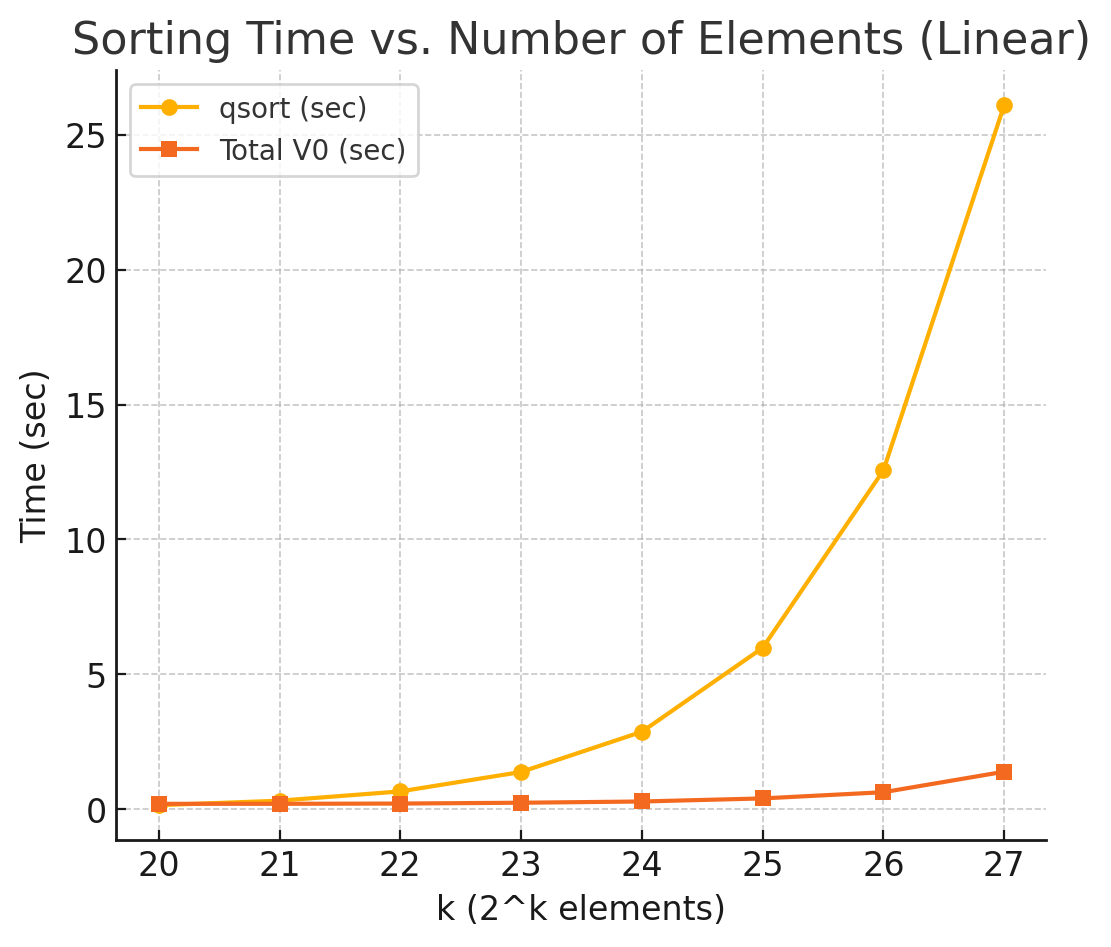
\includegraphics[width=0.5\linewidth]{plots/plot1_qsort_v0_times.png}
    \caption{qsort - total V0 times}
\end{figure}


Next, we present a diagram that compares the total execution time and the internal execution time of the \texttt{V0} implementation. This visualization helps us better understand the additional overhead introduced by memory transfers between the host and the device.

As evident from the diagram, this overhead increases for larger dataset sizes. This behavior is expected, as the memory copy operation exhibits linear complexity with respect to the number of elements. Consequently, for larger datasets (\( 2^{27} \) elements), the data transfer time becomes a more significant portion of the total execution time.

\begin{figure}[!h]
    \centering
    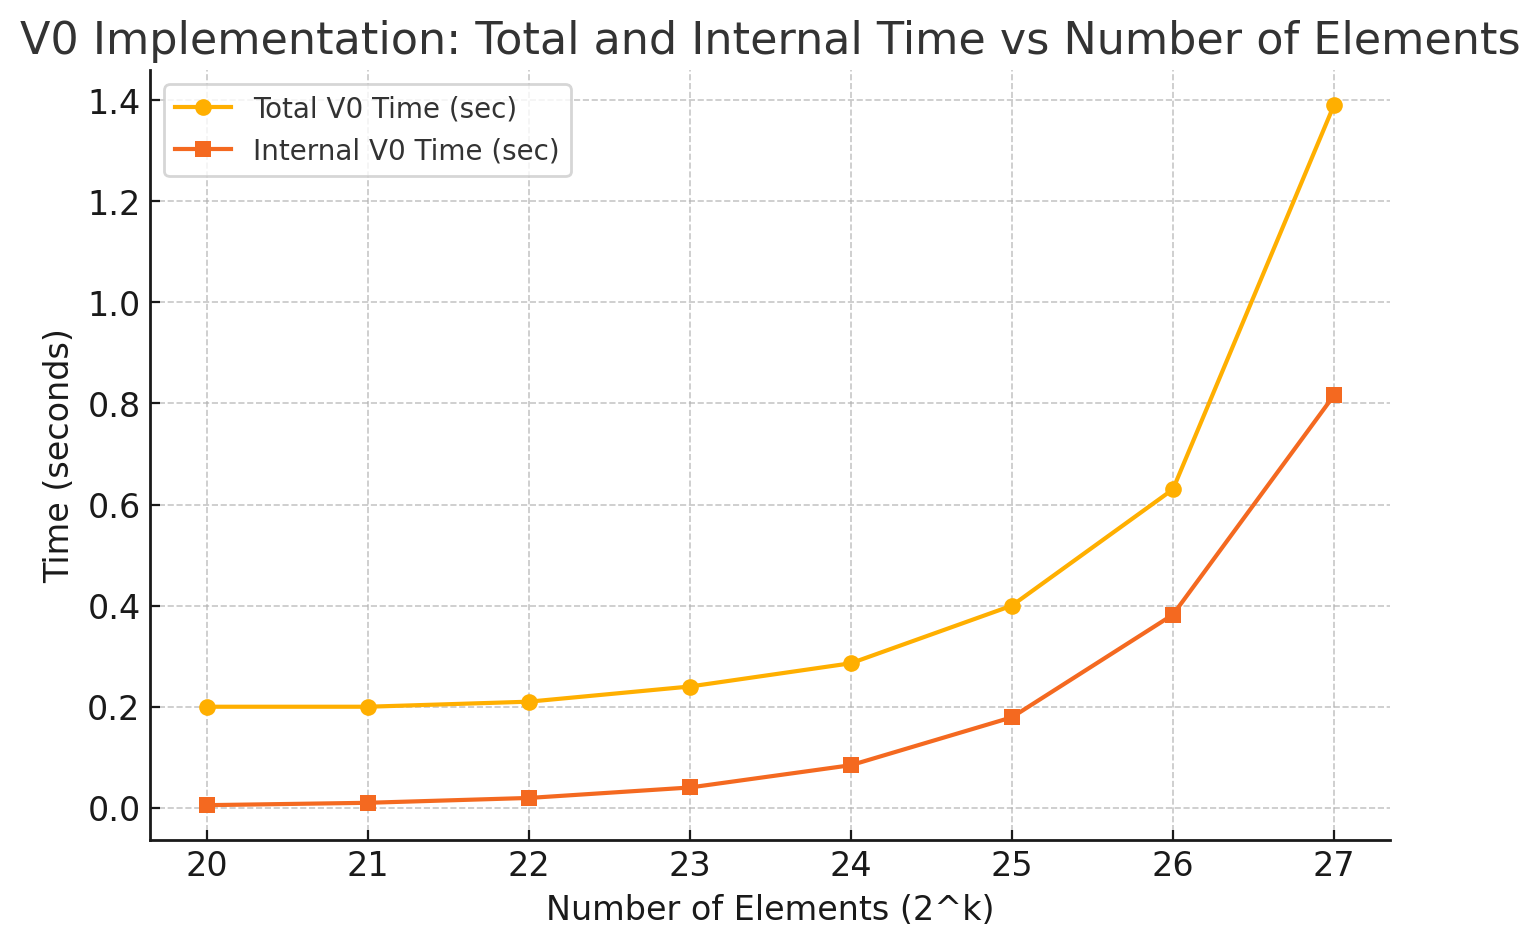
\includegraphics[width=0.65\linewidth]{plots/plot2_v0_total_and_internal.png}
    \caption{Bitonic Sort V0: Total \& Internal time}
\end{figure}


Lastly|after illustrating the difference between the internal and total execution times|we proceed to compare the internal execution times of all our implementations. We choose to present the pure sorting times (internal) to better highlight the acceleration achieved through our optimizations.

As evidenced in the results, the \texttt{V0} implementation is the slowest, which aligns with our theoretical analysis. On the other hand, the \texttt{V2} implementation, leveraging both shared memory and reduced kernel calls, demonstrates the best performance among all versions.

\begin{figure}[!h]
    \centering
    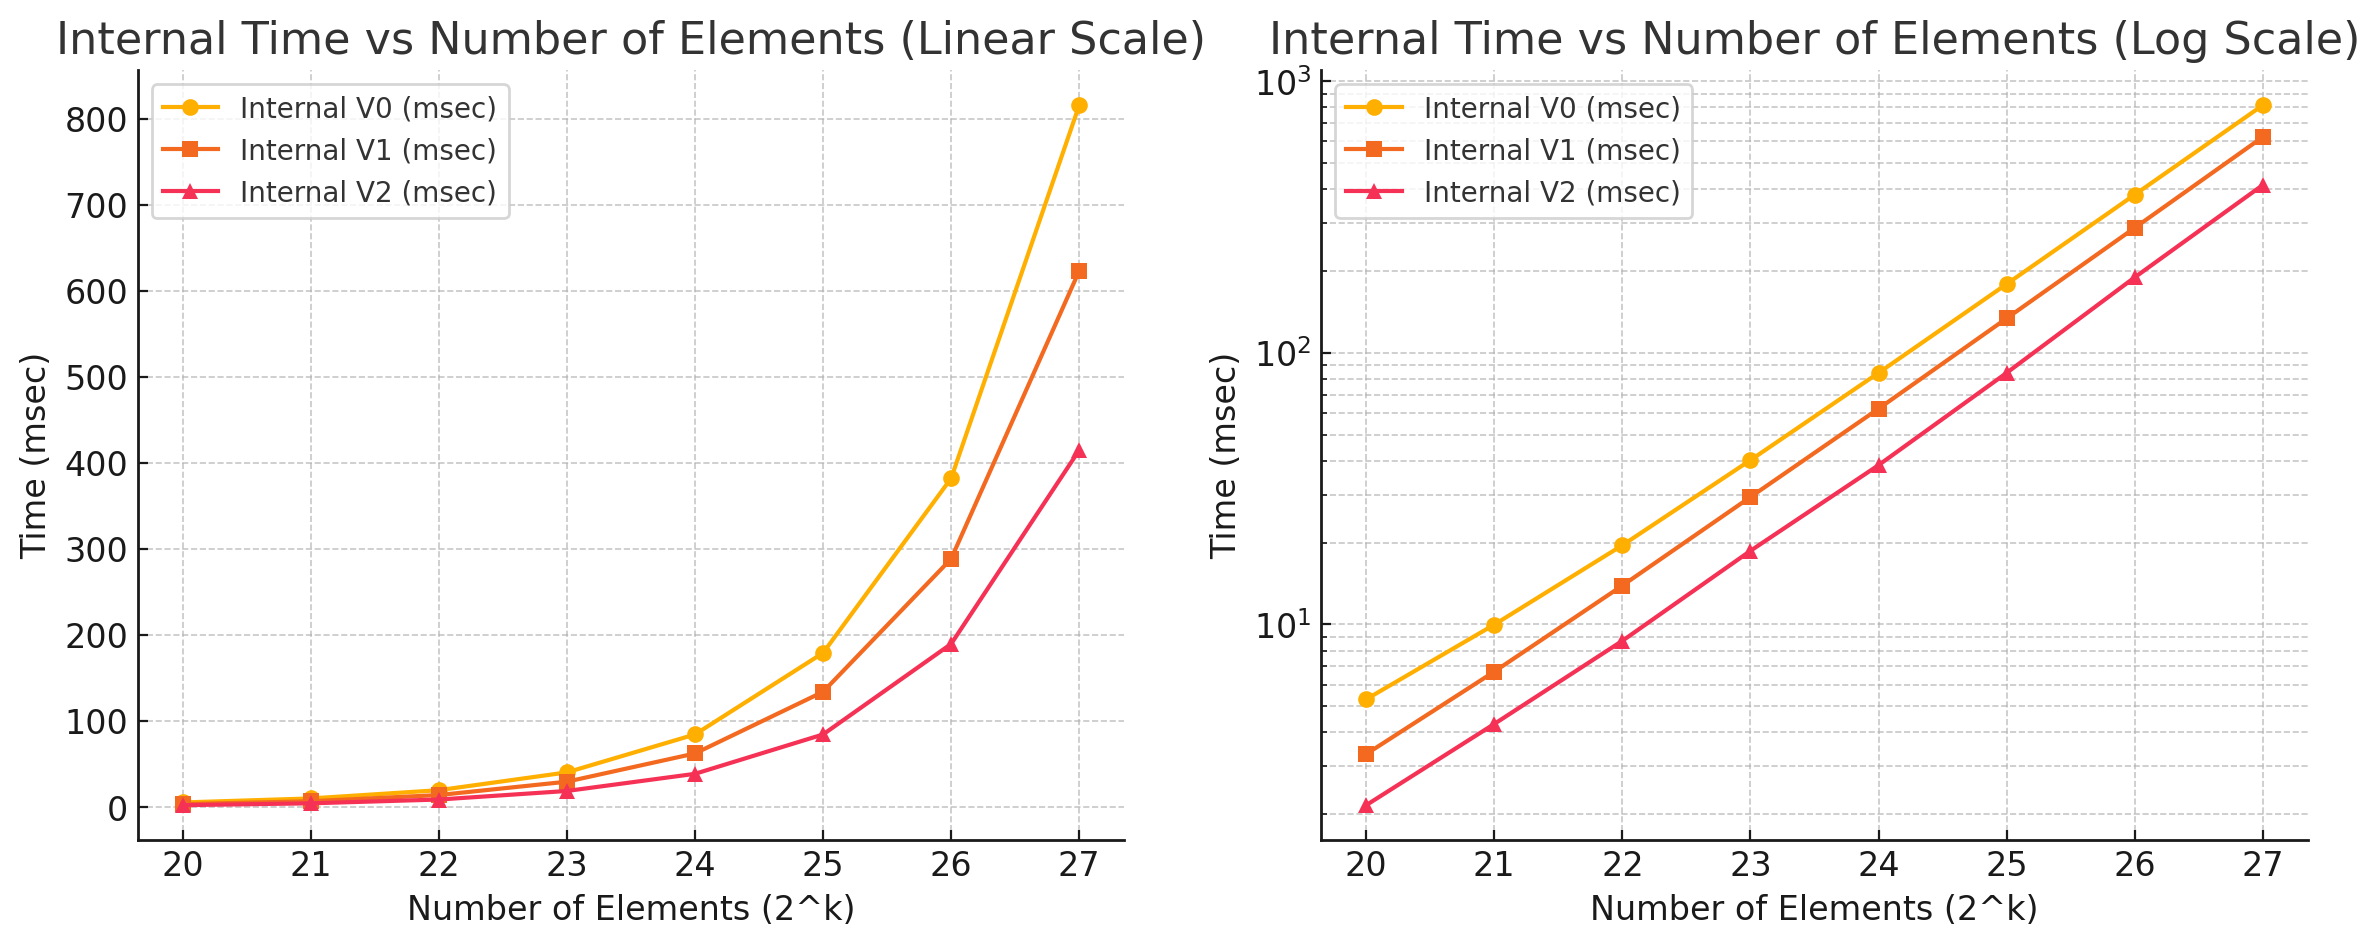
\includegraphics[width=1\linewidth]{plots/plot3_v0_v1_v2.png}
    \caption{Compare Versions' Times}
\end{figure}

\newpage

\end{document}